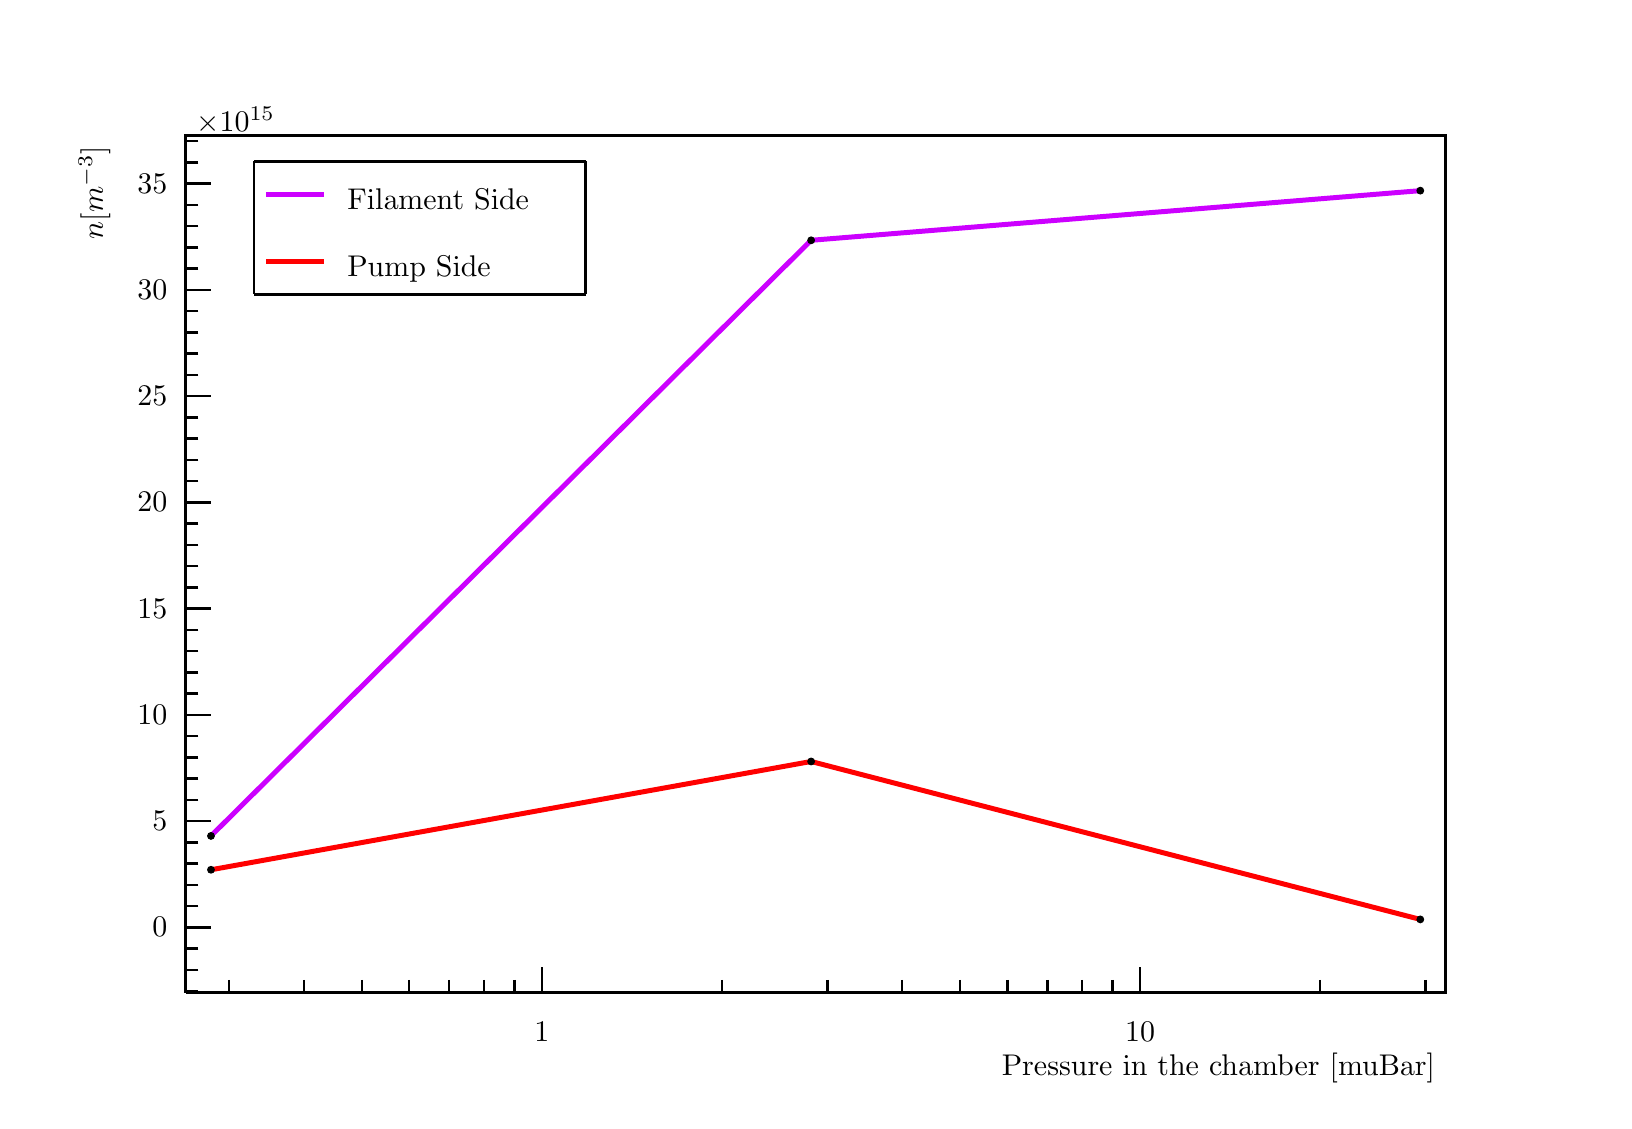
\begin{tikzpicture}
\pgfdeclareplotmark{cross} {
\pgfpathmoveto{\pgfpoint{-0.3\pgfplotmarksize}{\pgfplotmarksize}}
\pgfpathlineto{\pgfpoint{+0.3\pgfplotmarksize}{\pgfplotmarksize}}
\pgfpathlineto{\pgfpoint{+0.3\pgfplotmarksize}{0.3\pgfplotmarksize}}
\pgfpathlineto{\pgfpoint{+1\pgfplotmarksize}{0.3\pgfplotmarksize}}
\pgfpathlineto{\pgfpoint{+1\pgfplotmarksize}{-0.3\pgfplotmarksize}}
\pgfpathlineto{\pgfpoint{+0.3\pgfplotmarksize}{-0.3\pgfplotmarksize}}
\pgfpathlineto{\pgfpoint{+0.3\pgfplotmarksize}{-1.\pgfplotmarksize}}
\pgfpathlineto{\pgfpoint{-0.3\pgfplotmarksize}{-1.\pgfplotmarksize}}
\pgfpathlineto{\pgfpoint{-0.3\pgfplotmarksize}{-0.3\pgfplotmarksize}}
\pgfpathlineto{\pgfpoint{-1.\pgfplotmarksize}{-0.3\pgfplotmarksize}}
\pgfpathlineto{\pgfpoint{-1.\pgfplotmarksize}{0.3\pgfplotmarksize}}
\pgfpathlineto{\pgfpoint{-0.3\pgfplotmarksize}{0.3\pgfplotmarksize}}
\pgfpathclose
\pgfusepathqstroke
}
\pgfdeclareplotmark{cross*} {
\pgfpathmoveto{\pgfpoint{-0.3\pgfplotmarksize}{\pgfplotmarksize}}
\pgfpathlineto{\pgfpoint{+0.3\pgfplotmarksize}{\pgfplotmarksize}}
\pgfpathlineto{\pgfpoint{+0.3\pgfplotmarksize}{0.3\pgfplotmarksize}}
\pgfpathlineto{\pgfpoint{+1\pgfplotmarksize}{0.3\pgfplotmarksize}}
\pgfpathlineto{\pgfpoint{+1\pgfplotmarksize}{-0.3\pgfplotmarksize}}
\pgfpathlineto{\pgfpoint{+0.3\pgfplotmarksize}{-0.3\pgfplotmarksize}}
\pgfpathlineto{\pgfpoint{+0.3\pgfplotmarksize}{-1.\pgfplotmarksize}}
\pgfpathlineto{\pgfpoint{-0.3\pgfplotmarksize}{-1.\pgfplotmarksize}}
\pgfpathlineto{\pgfpoint{-0.3\pgfplotmarksize}{-0.3\pgfplotmarksize}}
\pgfpathlineto{\pgfpoint{-1.\pgfplotmarksize}{-0.3\pgfplotmarksize}}
\pgfpathlineto{\pgfpoint{-1.\pgfplotmarksize}{0.3\pgfplotmarksize}}
\pgfpathlineto{\pgfpoint{-0.3\pgfplotmarksize}{0.3\pgfplotmarksize}}
\pgfpathclose
\pgfusepathqfillstroke
}
\pgfdeclareplotmark{newstar} {
\pgfpathmoveto{\pgfqpoint{0pt}{\pgfplotmarksize}}
\pgfpathlineto{\pgfqpointpolar{44}{0.5\pgfplotmarksize}}
\pgfpathlineto{\pgfqpointpolar{18}{\pgfplotmarksize}}
\pgfpathlineto{\pgfqpointpolar{-20}{0.5\pgfplotmarksize}}
\pgfpathlineto{\pgfqpointpolar{-54}{\pgfplotmarksize}}
\pgfpathlineto{\pgfqpointpolar{-90}{0.5\pgfplotmarksize}}
\pgfpathlineto{\pgfqpointpolar{234}{\pgfplotmarksize}}
\pgfpathlineto{\pgfqpointpolar{198}{0.5\pgfplotmarksize}}
\pgfpathlineto{\pgfqpointpolar{162}{\pgfplotmarksize}}
\pgfpathlineto{\pgfqpointpolar{134}{0.5\pgfplotmarksize}}
\pgfpathclose
\pgfusepathqstroke
}
\pgfdeclareplotmark{newstar*} {
\pgfpathmoveto{\pgfqpoint{0pt}{\pgfplotmarksize}}
\pgfpathlineto{\pgfqpointpolar{44}{0.5\pgfplotmarksize}}
\pgfpathlineto{\pgfqpointpolar{18}{\pgfplotmarksize}}
\pgfpathlineto{\pgfqpointpolar{-20}{0.5\pgfplotmarksize}}
\pgfpathlineto{\pgfqpointpolar{-54}{\pgfplotmarksize}}
\pgfpathlineto{\pgfqpointpolar{-90}{0.5\pgfplotmarksize}}
\pgfpathlineto{\pgfqpointpolar{234}{\pgfplotmarksize}}
\pgfpathlineto{\pgfqpointpolar{198}{0.5\pgfplotmarksize}}
\pgfpathlineto{\pgfqpointpolar{162}{\pgfplotmarksize}}
\pgfpathlineto{\pgfqpointpolar{134}{0.5\pgfplotmarksize}}
\pgfpathclose
\pgfusepathqfillstroke
}
\definecolor{c}{rgb}{1,1,1};
\draw [color=c, fill=c] (0,0) rectangle (20,13.6103);
\draw [color=c, fill=c] (2,1.36103) rectangle (18,12.2493);
\definecolor{c}{rgb}{0,0,0};
\draw [c,line width=0.9] (2,1.36103) -- (2,12.2493) -- (18,12.2493) -- (18,1.36103) -- (2,1.36103);
\definecolor{c}{rgb}{1,1,1};
\draw [color=c, fill=c] (2,1.36103) rectangle (18,12.2493);
\definecolor{c}{rgb}{0,0,0};
\draw [c,line width=0.9] (2,1.36103) -- (2,12.2493) -- (18,12.2493) -- (18,1.36103) -- (2,1.36103);
\draw [c,line width=0.9] (2,1.36103) -- (18,1.36103);
\draw [c,line width=0.9] (2.55171,1.52436) -- (2.55171,1.36103);
\draw [c,line width=0.9] (3.50076,1.52436) -- (3.50076,1.36103);
\draw [c,line width=0.9] (4.23689,1.52436) -- (4.23689,1.36103);
\draw [c,line width=0.9] (4.83836,1.52436) -- (4.83836,1.36103);
\draw [c,line width=0.9] (5.34689,1.52436) -- (5.34689,1.36103);
\draw [c,line width=0.9] (5.78741,1.52436) -- (5.78741,1.36103);
\draw [c,line width=0.9] (6.17597,1.52436) -- (6.17597,1.36103);
\draw [c,line width=0.9] (6.52354,1.68768) -- (6.52354,1.36103);
\draw [anchor=base] (6.52354,0.745165) node[scale=1.08185, color=c, rotate=0]{1};
\draw [c,line width=0.9] (8.81019,1.52436) -- (8.81019,1.36103);
\draw [c,line width=0.9] (10.1478,1.52436) -- (10.1478,1.36103);
\draw [c,line width=0.9] (11.0968,1.52436) -- (11.0968,1.36103);
\draw [c,line width=0.9] (11.833,1.52436) -- (11.833,1.36103);
\draw [c,line width=0.9] (12.4345,1.52436) -- (12.4345,1.36103);
\draw [c,line width=0.9] (12.943,1.52436) -- (12.943,1.36103);
\draw [c,line width=0.9] (13.3835,1.52436) -- (13.3835,1.36103);
\draw [c,line width=0.9] (13.7721,1.52436) -- (13.7721,1.36103);
\draw [c,line width=0.9] (14.1196,1.68768) -- (14.1196,1.36103);
\draw [anchor=base] (14.1196,0.745165) node[scale=1.08185, color=c, rotate=0]{10};
\draw [c,line width=0.9] (16.4063,1.52436) -- (16.4063,1.36103);
\draw [c,line width=0.9] (17.7439,1.52436) -- (17.7439,1.36103);
\draw [anchor= east] (18,0.4) node[scale=1.08185, color=c, rotate=0]{Pressure in the chamber [muBar]};
\draw [c,line width=0.9] (2,1.36103) -- (2,12.2493);
\draw [c,line width=0.9] (2.32,2.19216) -- (2,2.19216);
\draw [c,line width=0.9] (2.16,2.46202) -- (2,2.46202);
\draw [c,line width=0.9] (2.16,2.73189) -- (2,2.73189);
\draw [c,line width=0.9] (2.16,3.00175) -- (2,3.00175);
\draw [c,line width=0.9] (2.16,3.27161) -- (2,3.27161);
\draw [c,line width=0.9] (2.32,3.54148) -- (2,3.54148);
\draw [c,line width=0.9] (2.16,3.81134) -- (2,3.81134);
\draw [c,line width=0.9] (2.16,4.0812) -- (2,4.0812);
\draw [c,line width=0.9] (2.16,4.35107) -- (2,4.35107);
\draw [c,line width=0.9] (2.16,4.62093) -- (2,4.62093);
\draw [c,line width=0.9] (2.32,4.89079) -- (2,4.89079);
\draw [c,line width=0.9] (2.16,5.16066) -- (2,5.16066);
\draw [c,line width=0.9] (2.16,5.43052) -- (2,5.43052);
\draw [c,line width=0.9] (2.16,5.70038) -- (2,5.70038);
\draw [c,line width=0.9] (2.16,5.97024) -- (2,5.97024);
\draw [c,line width=0.9] (2.32,6.24011) -- (2,6.24011);
\draw [c,line width=0.9] (2.16,6.50997) -- (2,6.50997);
\draw [c,line width=0.9] (2.16,6.77983) -- (2,6.77983);
\draw [c,line width=0.9] (2.16,7.0497) -- (2,7.0497);
\draw [c,line width=0.9] (2.16,7.31956) -- (2,7.31956);
\draw [c,line width=0.9] (2.32,7.58942) -- (2,7.58942);
\draw [c,line width=0.9] (2.16,7.85929) -- (2,7.85929);
\draw [c,line width=0.9] (2.16,8.12915) -- (2,8.12915);
\draw [c,line width=0.9] (2.16,8.39901) -- (2,8.39901);
\draw [c,line width=0.9] (2.16,8.66888) -- (2,8.66888);
\draw [c,line width=0.9] (2.32,8.93874) -- (2,8.93874);
\draw [c,line width=0.9] (2.16,9.2086) -- (2,9.2086);
\draw [c,line width=0.9] (2.16,9.47847) -- (2,9.47847);
\draw [c,line width=0.9] (2.16,9.74833) -- (2,9.74833);
\draw [c,line width=0.9] (2.16,10.0182) -- (2,10.0182);
\draw [c,line width=0.9] (2.32,10.2881) -- (2,10.2881);
\draw [c,line width=0.9] (2.16,10.5579) -- (2,10.5579);
\draw [c,line width=0.9] (2.16,10.8278) -- (2,10.8278);
\draw [c,line width=0.9] (2.16,11.0976) -- (2,11.0976);
\draw [c,line width=0.9] (2.16,11.3675) -- (2,11.3675);
\draw [c,line width=0.9] (2.32,11.6374) -- (2,11.6374);
\draw [c,line width=0.9] (2.32,2.19216) -- (2,2.19216);
\draw [c,line width=0.9] (2.16,1.9223) -- (2,1.9223);
\draw [c,line width=0.9] (2.16,1.65243) -- (2,1.65243);
\draw [c,line width=0.9] (2.16,1.38257) -- (2,1.38257);
\draw [c,line width=0.9] (2.32,11.6374) -- (2,11.6374);
\draw [c,line width=0.9] (2.16,11.9072) -- (2,11.9072);
\draw [c,line width=0.9] (2.16,12.1771) -- (2,12.1771);
\draw [anchor= east] (1.9,2.19216) node[scale=1.08185, color=c, rotate=0]{0};
\draw [anchor= east] (1.9,3.54148) node[scale=1.08185, color=c, rotate=0]{5};
\draw [anchor= east] (1.9,4.89079) node[scale=1.08185, color=c, rotate=0]{10};
\draw [anchor= east] (1.9,6.24011) node[scale=1.08185, color=c, rotate=0]{15};
\draw [anchor= east] (1.9,7.58942) node[scale=1.08185, color=c, rotate=0]{20};
\draw [anchor= east] (1.9,8.93874) node[scale=1.08185, color=c, rotate=0]{25};
\draw [anchor= east] (1.9,10.2881) node[scale=1.08185, color=c, rotate=0]{30};
\draw [anchor= east] (1.9,11.6374) node[scale=1.08185, color=c, rotate=0]{35};
\draw [anchor=base west] (2,12.2969) node[scale=1.08185, color=c, rotate=0]{$\times10^{15}$};
\draw [anchor= east] (0.841547,12.2493) node[scale=1.08185, color=c, rotate=90]{$n [m^{-3}]$};
\definecolor{c}{rgb}{0.8,0,1};
\draw [c,line width=1.8] (2.32092,3.35244) -- (9.94269,10.9169) -- (17.6791,11.5473);
\definecolor{c}{rgb}{0,0,0};
\foreach \P in {(2.32092,3.35244), (9.94269,10.9169), (17.6791,11.5473)}{\draw[mark options={color=c,fill=c},mark size=1.201201pt,mark=*] plot coordinates {\P};}
\definecolor{c}{rgb}{1,0,0};
\draw [c,line width=1.8] (2.32092,2.92264) -- (9.94269,4.29799) -- (17.6791,2.29226);
\definecolor{c}{rgb}{0,0,0};
\foreach \P in {(2.32092,2.92264), (9.94269,4.29799), (17.6791,2.29226)}{\draw[mark options={color=c,fill=c},mark size=1.201201pt,mark=*] plot coordinates {\P};}
\definecolor{c}{rgb}{1,1,1};
\draw [color=c, fill=c] (2.86533,10.2292) rectangle (7.07736,11.9198);
\definecolor{c}{rgb}{0,0,0};
\draw [c,line width=0.9] (2.86533,10.2292) -- (7.07736,10.2292);
\draw [c,line width=0.9] (7.07736,10.2292) -- (7.07736,11.9198);
\draw [c,line width=0.9] (7.07736,11.9198) -- (2.86533,11.9198);
\draw [c,line width=0.9] (2.86533,11.9198) -- (2.86533,10.2292);
\draw [anchor=base west] (3.91834,11.3069) node[scale=1.08185, color=c, rotate=0]{Filament Side};
\definecolor{c}{rgb}{0.8,0,1};
\draw [c,line width=1.8] (3.02328,11.4971) -- (3.76039,11.4971);
\definecolor{c}{rgb}{0,0,0};
\draw [anchor=base west] (3.91834,10.4617) node[scale=1.08185, color=c, rotate=0]{Pump Side};
\definecolor{c}{rgb}{1,0,0};
\draw [c,line width=1.8] (3.02328,10.6519) -- (3.76039,10.6519);
\end{tikzpicture}
